% File: minimax_tree.tex
% Description: A hardcoded TikZ Minimax tree - not generic, not scalable at all.

\documentclass{standalone}
\usepackage{tikz}
\usetikzlibrary{arrows.meta, shapes.geometric}

\begin{document}
    
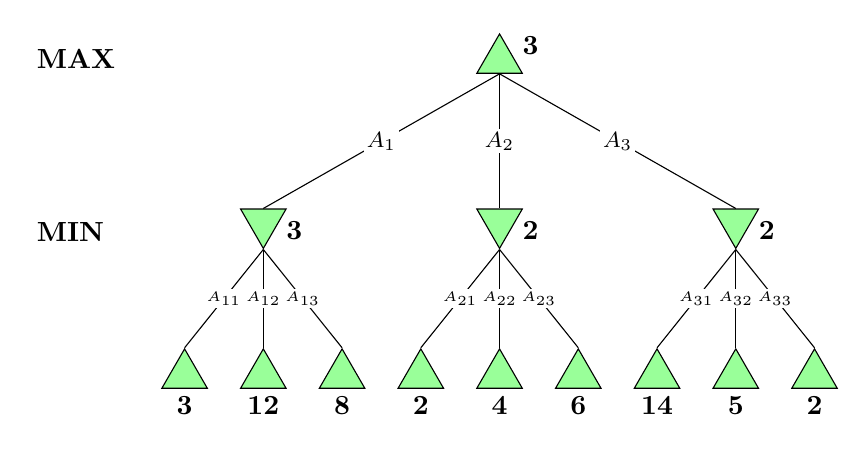
\begin{tikzpicture}[
    triUp/.style = {
        isosceles triangle,
        isosceles triangle apex angle = 60,
        draw,
        fill = green!40,
        minimum size = 5mm,
        shape border rotate = 120
    },
    triDown/.style = {
        isosceles triangle,
        isosceles triangle apex angle = 60,
        draw,
        fill = green!40,
        minimum size = 5mm,
        shape border rotate = 240
    },
    node distance = 2.6cm and 2cm,
    edgeLabel/.style = {font=\footnotesize, midway, fill=white, inner sep=1pt},
    valLabel/.style = {font=\bfseries, yshift=-4pt},
]

    % Root (MAX)
    \node[triUp] (root) at (0,0) {};
    \node[valLabel, xshift=5pt, yshift=10pt] at (root.east) {3};
    \node[anchor=south west,font=\bfseries] at (-6,-0.2) {MAX};
    
    % Second layer (MIN)
    \node[triDown] (L1) at (-3,-2) {};
    \node[triDown] (L2) at (0,-2)  {};
    \node[triDown] (L3) at (3,-2)  {};
    \node[valLabel, xshift=5pt] at (L1.east) {3};
    \node[valLabel, xshift=5pt] at (L2.east) {2};
    \node[valLabel, xshift=5pt] at (L3.east) {2};
    \node[anchor=south west,font=\bfseries] at (-6,-2.4) {MIN};
    
    % Third layer (MAX)
    % Left subtree
    \node[triUp] (L11) at (-4,-4) {};
    \node[triUp] (L12) at (-3,-4) {};
    \node[triUp] (L13) at (-2,-4) {};
    \node[valLabel, yshift=-2pt] at (L11.south) {3};
    \node[valLabel, yshift=-2pt] at (L12.south) {12};
    \node[valLabel, yshift=-2pt] at (L13.south) {8};
    
    % Middle subtree
    \node[triUp] (L21) at (-1,-4) {};
    \node[triUp] (L22) at (0,-4) {};
    \node[triUp] (L23) at (1,-4) {};
    \node[valLabel, yshift=-2pt] at (L21.south) {2};
    \node[valLabel, yshift=-2pt] at (L22.south) {4};
    \node[valLabel, yshift=-2pt] at (L23.south) {6};
    
    % Right subtree
    \node[triUp] (L31) at (2, -4) {};
    \node[triUp] (L32) at (3,-4) {};
    \node[triUp] (L33) at (4,-4) {};
    \node[valLabel, yshift=-2pt] at (L31.south) {14};
    \node[valLabel, yshift=-2pt] at (L32.south) {5};
    \node[valLabel, yshift=-2pt] at (L33.south) {2};
    
    % Edges
    % Root to second layer
    \draw (root.south) -- (L1.north) node[edgeLabel] {$A_1$};
    \draw (root.south) -- (L2.north) node[edgeLabel] {$A_2$};
    \draw (root.south) -- (L3.north) node[edgeLabel] {$A_3$};
    
    % Second layer to third layer
    \draw (L1.south) -- (L11.north) node[edgeLabel, font=\tiny] {$A_{11}$};
    \draw (L1.south) -- (L12.north) node[edgeLabel, font=\tiny] {$A_{12}$};
    \draw (L1.south) -- (L13.north) node[edgeLabel, font=\tiny] {$A_{13}$};
    
    \draw (L2.south) -- (L21.north) node[edgeLabel, font=\tiny] {$A_{21}$};
    \draw (L2.south) -- (L22.north) node[edgeLabel, font=\tiny] {$A_{22}$};
    \draw (L2.south) -- (L23.north) node[edgeLabel, font=\tiny] {$A_{23}$};
    
    \draw (L3.south) -- (L31.north) node[edgeLabel, font=\tiny] {$A_{31}$};
    \draw (L3.south) -- (L32.north) node[edgeLabel, font=\tiny] {$A_{32}$};
    \draw (L3.south) -- (L33.north) node[edgeLabel, font=\tiny] {$A_{33}$};
\end{tikzpicture}

\end{document}
